\documentclass{standalone}
\usepackage{tikz}
\usetikzlibrary{calc, shapes.geometric, arrows.meta, positioning, fit, decorations.pathreplacing}

\begin{document}
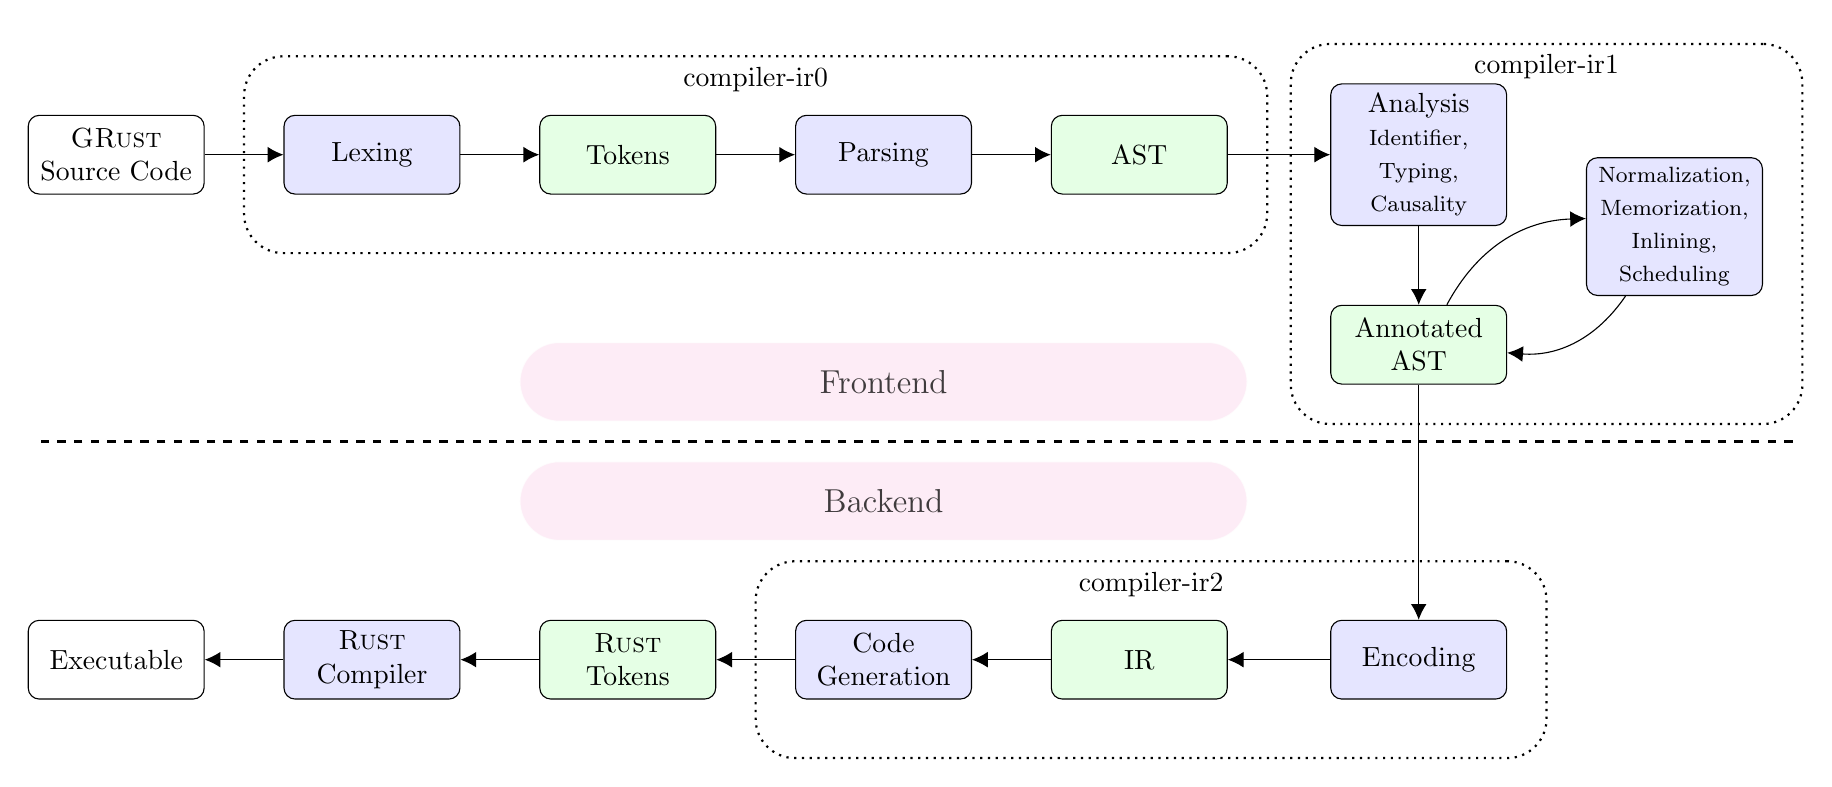
\begin{tikzpicture}[
    node distance=1cm,
    every node/.style={
            rectangle,
            rounded corners,
            draw,
            text width=2cm,
            text centered,
            minimum height=1cm
        },
    arrow/.style={-{Latex[length=2mm, width=2mm]}},
    crate_border/.style={
            dotted,
            thick,
            rounded corners=5mm,
            inner sep=5mm,
            minimum height=2.5cm,
            minimum width=3.5cm
        },
    process_block/.style={fill=blue!10},
    data_block/.style={fill=green!10},
    label_block/.style={
            rounded corners=5mm,
            draw = white,
            nearly opaque,
            fill=magenta!10,
            text width=9cm,
        }
    ]

    % --- Input ---
    \node (grust_code) {\textsc{GRust} Source Code};

    % --- Frontend ---
    \node (lexer) [process_block, right=of grust_code] {Lexing};
    \node (tokens) [data_block, right=of lexer] {Tokens};
    \node (parser) [process_block, right=of tokens] {Parsing};
    \node (ast) [data_block, right=of parser] {AST};
    \node (analysis) [process_block, right=1.3cm of ast] {Analysis {\footnotesize Identifier, Typing, Causality}};
    \node (annotated_ast) [data_block, below=of analysis] {Annotated AST};
    \node (normalization) [process_block, right=of annotated_ast, yshift=1.5cm] {\footnotesize Normalization, Memorization, Inlining, Scheduling};

    % --- Backend ---
    \node (encoding) [process_block, below=5cm of analysis] {Encoding};
    \node (target_ir) [data_block, left=1.3cm of encoding] {IR};
    \node (codegen) [process_block, left=of target_ir] {Code Generation};
    \node (rust_tokens) [data_block, left=of codegen] {\textsc{Rust} Tokens};
    \node (rustc) [process_block, left=of rust_tokens] {\textsc{Rust} Compiler};
    \node (executable) [left=of rustc] {Executable};

    % --- Arrows ---
    \draw[arrow] (grust_code) -- (lexer);
    \draw[arrow] (lexer) -- (tokens);
    \draw[arrow] (tokens) -- (parser);
    \draw[arrow] (parser) -- (ast);
    \draw[arrow] (ast) -- (analysis);
    \draw[arrow] (analysis) -- (annotated_ast);
    \draw[arrow] (annotated_ast) to [bend left=30] (normalization);
    \draw[arrow] (normalization) to [bend left=30] (annotated_ast);
    \draw[arrow] (annotated_ast) -- (encoding);
    \draw[arrow] (encoding) -- (target_ir);
    \draw[arrow] (target_ir) -- (codegen);
    \draw[arrow] (codegen) -- (rust_tokens);
    \draw[arrow] (rust_tokens) -- (rustc);
    \draw[arrow] (rustc) -- (executable);

    % --- GRust Compiler Crates (Overlapping with Frontend/Backend) ---
    \node[crate_border,
        fit=(lexer) (tokens) (parser) (ast),
        label={[anchor=north, yshift=0.2cm]north:compiler-ir0}] (ir0_border) {};

    \node[crate_border,
        fit=(analysis) (annotated_ast) (normalization),
        label={[anchor=north, yshift=0.2cm]north:compiler-ir1}] (ir1_border) {};

    \node[crate_border,
        fit=(encoding) (target_ir) (codegen),
        label={[anchor=north, yshift=0.2cm]north:compiler-ir2}] (ir2_border) {};

    % --- Frontend/Backend Labels ---
    \node [label_block, above=1cm of codegen, font=\large] (backend) {Backend};
    \node [label_block, above=0.5cm of backend, font=\large] (frontend) {Frontend};

    % --- Dashed Line ---
    \coordinate (P) at ($(backend)!0.5!(frontend)$);
    \draw[dashed, thick]
    let \p1 = (P) in
    let \p2 = (normalization) in
    let \p3 = (executable) in
    ($(0,\y1)+(\x2+1.5cm,0)$) -- ($(0,\y1)+(\x3-1cm,0)$);

\end{tikzpicture}
\end{document}
